\subsection{ORBITS}

DEFINITION 5. Let G be a group, E a G-set and \(x \in G\) . An element \(y \in E\) is conjugate to x under the operation of G if there exists an element \(\alpha \in G\) such that \(y = \alpha x\) . The set of conjugate elements of x is called the orbit of x in E.

The relation ``y is conjugate to x'' is an equivalence relation. For x = ex; if \(y = \alpha x\) , then \(x = \alpha^{-1} y\) ; if \(y = \alpha x\) and \(z = \beta y\) , then \(z = \beta \alpha x\) . The orbits are the equivalence classes under this relation.

A subset X of E is stable if and only if it is saturated with respect to the relation of conjugation.

The mapping \(\alpha\mapsto\alpha x\) of G into E is sometimes called the orbital mapping defined by x. It is a G-morphism of G (with the operation of G on itself by left translation) into E. The image G.x of G under this mapping is the orbit of x.

G is said to operate freely on E if, for all \(x \in E\) , the orbital mapping defined by x is injective or also if the mapping \((g, x) \mapsto (gx, x)\) of G × E into E × E is injective.

Examples. (1) Let G be a group and consider the operation of G on itself by inner automorphisms. Two elements of G which are conjugate under this operation are called conjugate under inner automorphisms or simply conjugate. The orbits are called conjugacy classes. Similarly, two subsets H and \(H'\) of G are called conjugate if there exists an element \(\alpha \in G\) such that \(H' = \alpha \cdot H \cdot \alpha^{-1}\) , that is if they are conjugate under the extension to \(\mathfrak{P}(G)\) of the operation of G on itself by inner automorphisms.

\begin{enumerate}
\def\labelenumi{(\arabic{enumi})}
\setcounter{enumi}{1}
\tightlist
\item
  *In the space \(\mathbf{R}^n\) , the orbit of a point \(x\) under the action of the orthogonal group \(\mathbf{O}(n, \mathbf{R})\) is the Euclidean sphere of radius \(\| x \|\) .
\end{enumerate}

The stabilizers of two conjugate elements of E are conjugate subgroups of G (no. 2, Proposition 2).

The quotient set of E under the relation of conjugation is the set of orbits of E; it is sometimes denoted by E/G or \(G\backslash E\). (Sometimes the notation E/G is reserved for the case where E is a right G-set and the notation \(G\backslash E\) for the case where E is a left G-set.)

Let G be a group operating on a set E on the right. Let H be a normal subgroup of G. The group G operates on E/H on the right, the corresponding law of right action being \((xH, g) \mapsto xHg = xgH\) ; under this operation, H operates trivially, whence a right operation of G/H on E/H. Let \(\phi\) be the canonical mapping of E/H onto E/G; the inverse images under \(\phi\) of the points of E/G are the orbits of G (or of G/H) in E/H. Hence \(\phi\) defines when passing to the quotient a bijection, called canonical, of \((\mathrm{E}/\mathrm{H})/\mathrm{G} = (\mathrm{E}/\mathrm{H})/(\mathrm{G}/\mathrm{H})\) onto E/G.

Let G (resp. H) be a group operating on a set E on the left (resp. right). Suppose that the actions of G and H on E commute, that is

\[
(g. x). h = g. (x. h) \quad \text { for } g \in \mathrm{G}, x \in \mathrm{E} \text { and } h \in \mathrm{H}.
\]

The action of H on E is also a left operation of the opposite group \(H^{0}\) to H. It then follows from § 4, no. 9, Proposition 12 that the mapping which associates with the element \((g, h) \in G \times H^{0}\) the mapping \(x \mapsto g \cdot x \cdot h\) of E into itself is a left operation of \(G \times H^{0}\) on E. The orbit of an element \(x \in E\) under this operation is the set GxH. The set of these orbits is denoted by \(G\backslash E/H\). On the other hand, the operation of G (resp. H) is compatible with the relation of conjugation with respect to the operation of H (resp. G) and the set of orbits \(G\backslash(E/H)\) (resp. \((G\backslash E)/H\)) is identified with \(G\backslash E/H\): in the diagram

\pandocbounded{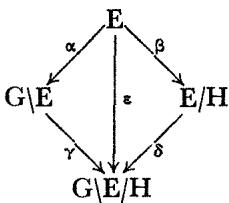
\includegraphics[keepaspectratio]{images/part001_b92675b5.jpg}}

(where \(\alpha, \beta, \gamma, \delta, \varepsilon\) denote the canonical mappings of taking quotients), \(\gamma \circ \alpha = \delta \circ \beta = \varepsilon\) .

Let G be a group and H a subgroup of G. Consider the right operation of H on G by right translation (no. 1, Example 2). The set of orbits G/H is the set of left cosets modulo H; note that G operates on G/H on the left by the law \((g, xH) \mapsto gxH\) (cf.~no. 5). Similarly, the set of right cosets modulo H is the set \(H\backslash G\) of orbits of the left operation of H on G by left translation. If K is a subgroup of G containing H and \(\Gamma\) is a left (resp. right) coset modulo H, then \(\Gamma K\) (resp. \(K\Gamma\) ) is a left (resp. right) coset modulo K. The mapping \(\Gamma \mapsto \Gamma K\) (resp. \(\Gamma \mapsto K\Gamma\) ) is called the canonical mapping of G/H into G/K (resp. of \(H\backslash G\) into \(K\backslash G\)). It is surjective.

Let G be a group and H and K two subgroups of G. Let H operate on G on the left by left translation and K on the right by right translation; these two operations commute, which allows us to consider the set \(H\backslash G/K\). The elements of \(H\backslash G/K\) are called the double cosets of G modulo H and K. When K = H, we simply say double cosets modulo H. For the canonical mapping of G/H onto \(H\backslash G/H\) to be a bijection, it is necessary and sufficient that H be a normal subgroup of G.

